\documentclass[12pt, a4paper] {ncc}

\usepackage[utf8] {inputenc}
\usepackage[T2A]{fontenc}
\usepackage[english, russian] {babel}
\let\proof\relax
\let\endproof\relax
\usepackage{amsthm}
\usepackage{amsmath}
\usepackage{amssymb}
\usepackage{listings}
\usepackage{hyperref}
\usepackage{color}
\usepackage{graphicx}
\usepackage{listings}
\usepackage{caption}
\graphicspath{ {./} }

\captionsetup{labelformat=empty,labelsep=none}

\lstset{
	basicstyle=\footnotesize,
	breakatwhitespace=false,
	breaklines=true,
	extendedchars=true,
	frame=single,
	keepspaces=true,
	keywordstyle=\bfseries,
	language=C,
	numbers=left,
	numbersep=5pt,
	numberstyle=\tiny,
	showspaces=false,
	showstringspaces=false,
	showtabs=false,
	stepnumber=1,
	stringstyle=\emph,
	tabsize=4
}
\lstset{extendedchars=\true}

\begin{document}


\textbf{Денис Ваксман, M3439}


\textbf{Курсовая работа по курсу "Введение в базы данных"}


\section{Модель сущность-связь}
По умолчанию все поля обязательные. \\
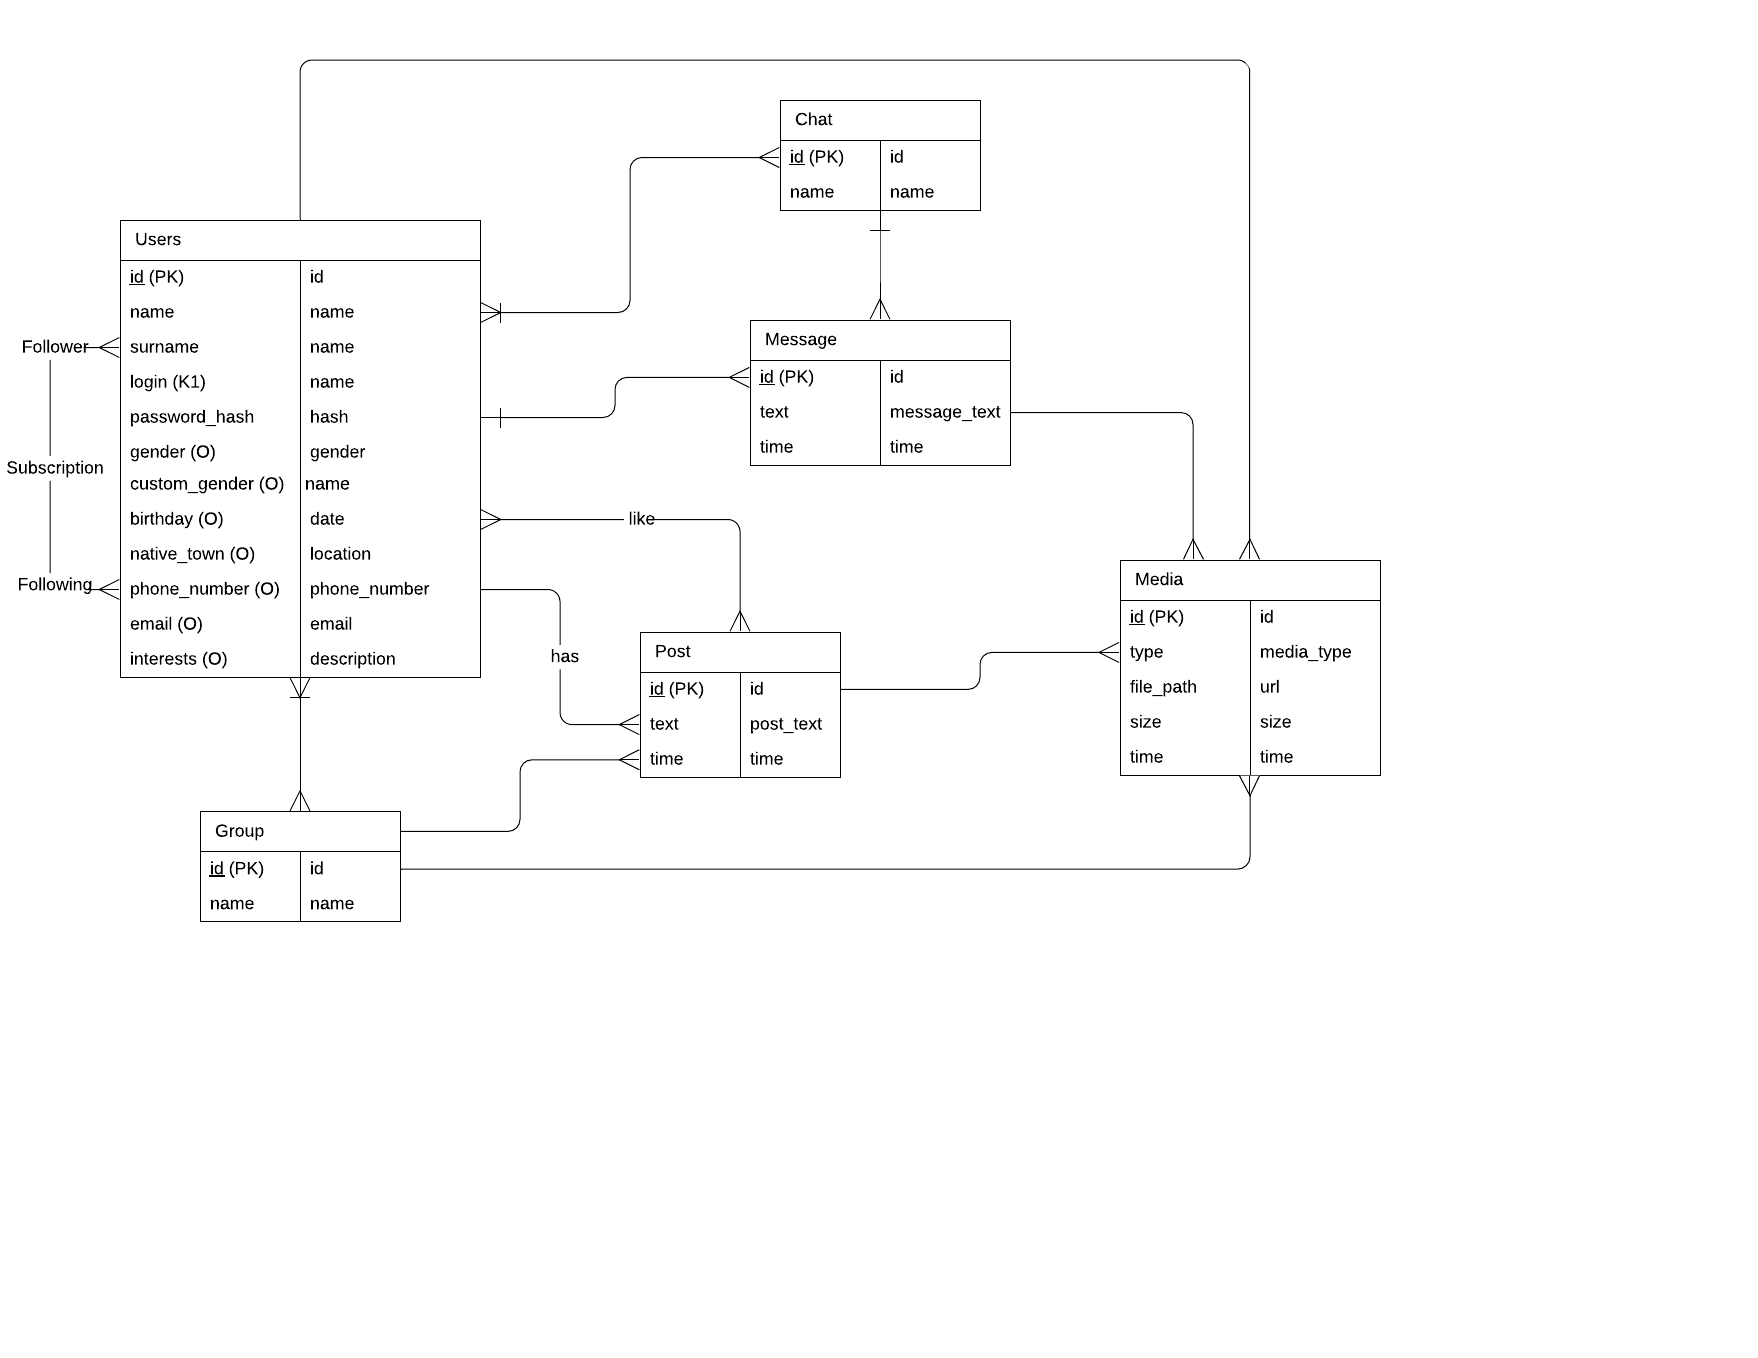
\includegraphics[scale=0.8]{rel.png}
\section{Физическая модель}
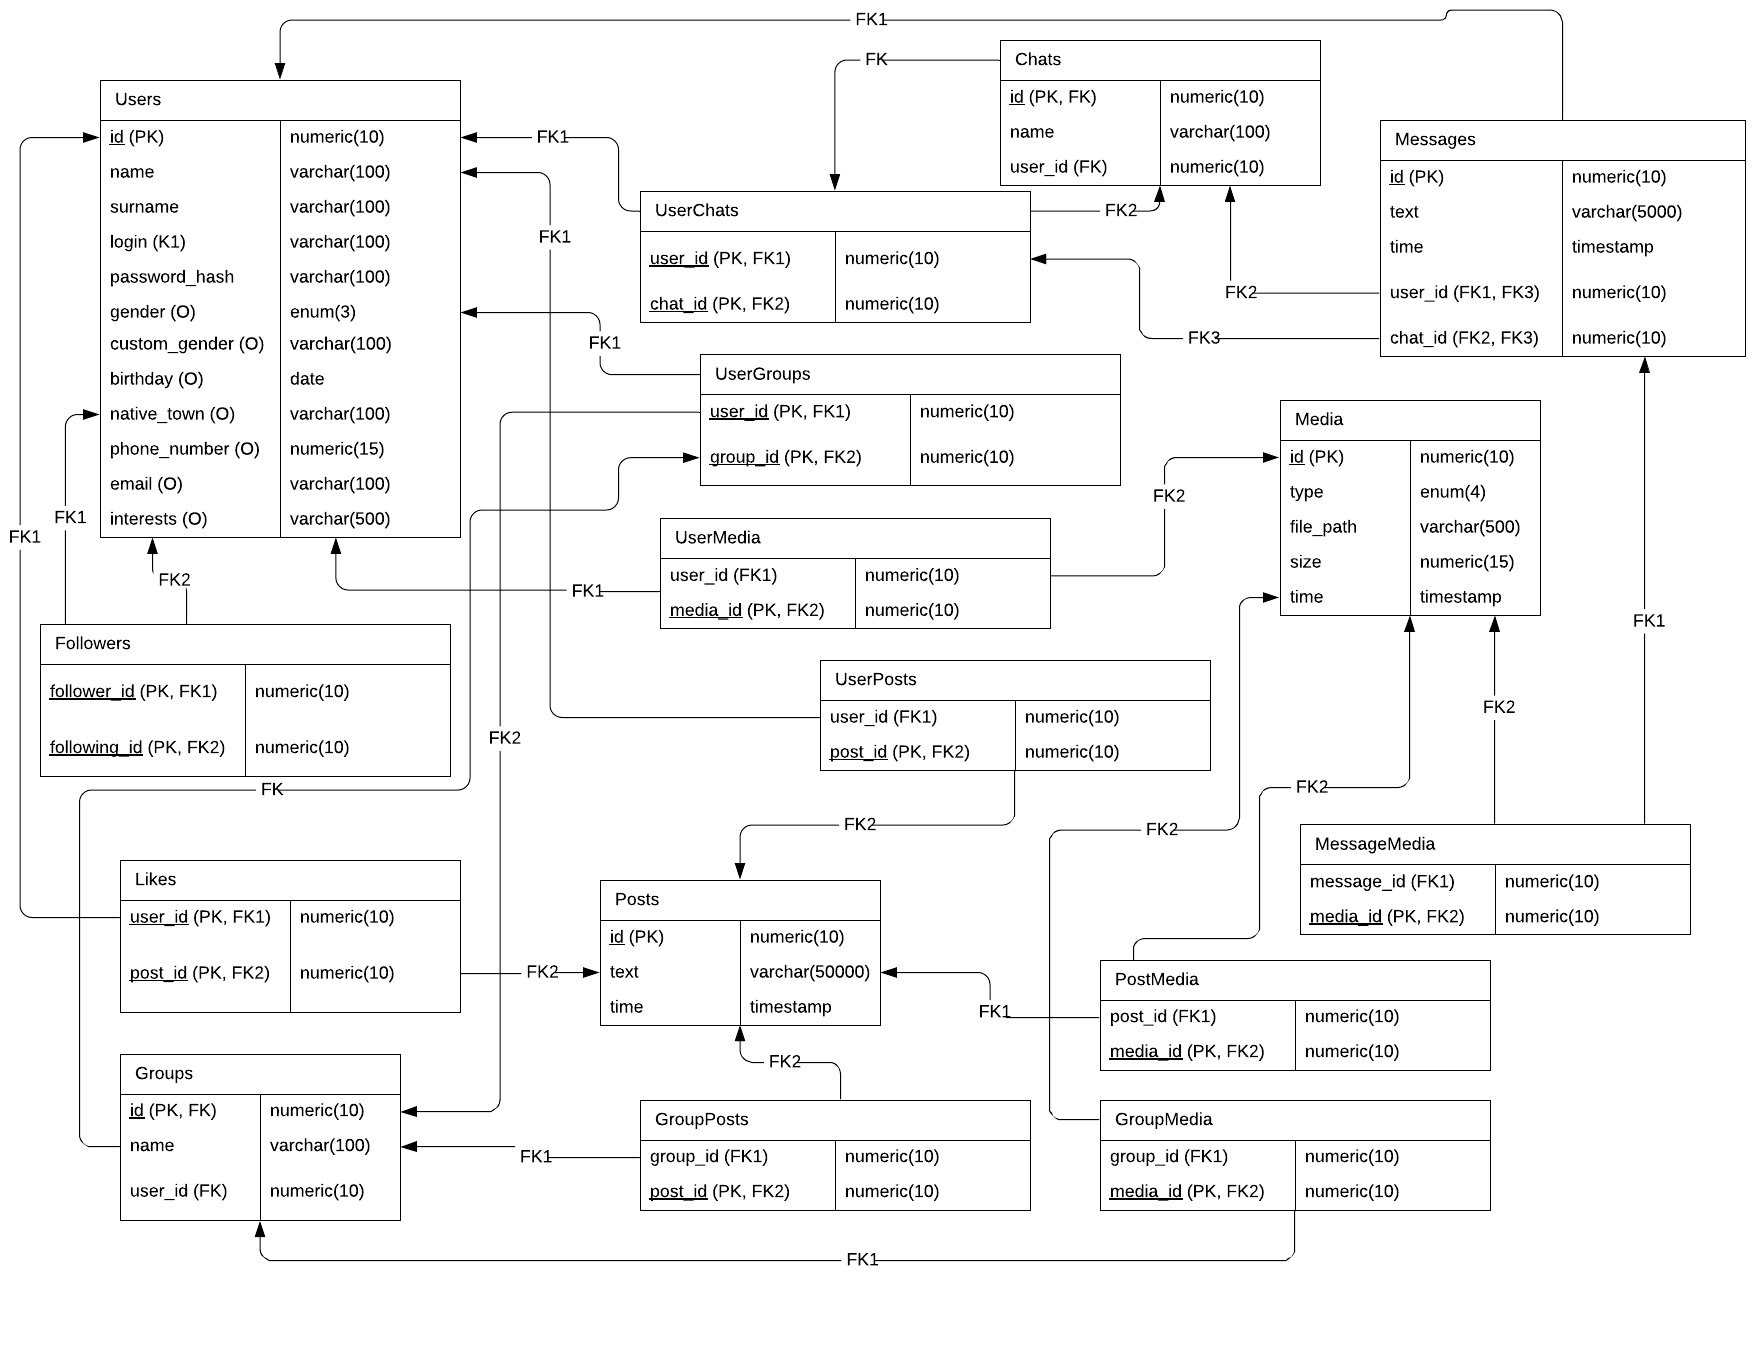
\includegraphics[scale=0.6]{phys.png}
\section{Нормализация}
\subsection{Функциональные зависимости}
\textbf{Media:}
\begin{itemize}
\item id $\rightarrow$ filePath
\item filePath $\rightarrow$ id
\item id $\rightarrow$ type
\item id $\rightarrow$ size
\item id $\rightarrow$ time
\end{itemize}
У следующих отношений пустое множество функциональных зависимостей:
\begin{itemize}
\item UserChats
\item UserGroups
\item Followers
\item Likes
\end{itemize}
У следующих отношений множество функциональных зависимостей имеет вид \\
$\{id \rightarrow A ~ | ~ \forall A \in \textit{attrs}, A \ne id\}$:
\begin{itemize}
\item Users
\item Chats
\item Messages
\item Groups
\item Posts
\item UserPosts
\item UserMedia
\item GroupPosts
\item GroupMedia
\item PostMedia
\item MessageMedia
\end{itemize}
\subsection{Нормальные формы}
Все отношения находятся в 5 НФ. Доказательство:\\
\textbf{Media}:
\begin{itemize}
\item 3 НФ: \\
т.к. все неключевые атрибуты непосредственно зависят от ключа
\item НФБК: \\
т.к. все ключи простые и 3НФ
\item 4НФ и 5НФ: \\
по теореме Дейта-Фейгина 1 (все ключи простые и НФБК)
\end{itemize}
\textbf{UserChats, UserGroups, Followers и Likes}:
\begin{itemize}
\item НФБК, так как пустое множество ФЗ ($\Rightarrow$ 3НФ)
\item Все отношения состоят из двух атрибутов $\Rightarrow$ имеют только тривиальные МЗ $\Rightarrow$ 4НФ
\item Так как атрибутов всего 2, возможно только одно нетривиальное разбиение: *\{X, Y\}.\\ 
Но при таком разбиении они не пересекаются $\Rightarrow$ это не ЗС $\Rightarrow$ 5НФ
\end{itemize}
\textbf{Оставшиеся} отношения имеют множество ФЗ вида \\
$\{id \rightarrow A ~ | ~ \forall A \in \textit{attrs}, A \ne id\}$:
\begin{itemize}
\item 3 НФ: \\
т.к. все неключевые атрибуты непосредственно зависят от ключа
\item НФБК: \\
т.к. все ключи простые и 3НФ
\item 4НФ и 5НФ: \\
по теореме Дейта-Фейгина 1 (все ключи простые и НФБК)
\end{itemize}
\section{Основные SQL запросы}
\subsection{Частые действия}
\begin{enumerate}
\item \textbf{Пользователь отправил в чат сообщение с картинкой} \\
Входные данные: \\
USER\_ID -- id пользователя\\
CHAT\_ID -- id чата\\
MSG\_TEXT -- текст сообщения\\
URL -- картинка\\
SIZE -- размер картинки
\lstinputlisting[language=sql]{../sql/actions/1.sql}
\item \textbf{Пользователь подал заявку в друзья другому пользователю} \\
FROM\_ID -- инциатор заявки \\
TO\_ID -- кому заявка
\lstinputlisting[language=sql]{../sql/actions/2.sql}
\item \textbf{Пользователь опубликовал пост} \\
Входные данные: USER\_ID, POST\_TEXT
\lstinputlisting[language=sql]{../sql/actions/3.sql}
\item \textbf{Пользователь лайкнул пост} \\
Входные данные: USER\_ID, POST\_ID
\lstinputlisting[language=sql]{../sql/actions/4.sql}
\item \textbf{Пользователь подписался на группу} \\
Входные данные: USER\_ID, GROUP\_ID
\lstinputlisting[language=sql]{../sql/actions/5.sql}
\item \textbf{Группа опубликовала пост} \\
Входные данные: GROUP\_ID, POST\_TEXT
\lstinputlisting[language=sql]{../sql/actions/6.sql}
\item \textbf{Пользователь загрузил фотографию} \\
Входные данные: USER\_ID, URL, SIZE
\lstinputlisting[language=sql]{../sql/actions/7.sql}
\item \textbf{Группа загрузила видеозапись} \\
Входные данные: GROUP\_ID, URL, SIZE
\lstinputlisting[language=sql]{../sql/actions/8.sql}
\item \textbf{Пользователь открыл ленту (получил все посты своих групп и подписок, кроме тех, которые уже лайкал)} \\
Входные данные: USER\_ID
\lstinputlisting[language=sql, tab=2]{../sql/actions/9.sql}
\item \textbf{Получить топ 20 интересных постов (20 постов с наибольшим количеством лайков от подписок)} \\
Входные данные: USER\_ID
\lstinputlisting[language=sql]{../sql/actions/10.sql}
\item \textbf{Получить общих друзей с другим пользователем} \\
Входные данные: USER\_ID, OTHER\_ID
\lstinputlisting[language=sql]{../sql/actions/11.sql}
\item \textbf{Получить 10 наиболее возможных знакомых (10 человек с наибольшим количеством общих друзей)} \\
Входные данные: USER\_ID \\
\lstinputlisting[language=sql]{../sql/actions/12.sql}
\item \textbf{Получить ранжированный список друзей (по количеству сообщений в смежных чатах)} \\
Входные данные: USER\_ID
\lstinputlisting[language=sql]{../sql/actions/13.sql}
\item \textbf{Получить ранжированный список групп (по количеству лайков от пользователя на постах этой группы)} \\
Входные данные: USER\_ID \\\\
\lstinputlisting[language=sql]{../sql/actions/14.sql}
\item \textbf{Получить список чатов в порядке времени последнего сообщения} \\
Входные данные: USER\_ID
\lstinputlisting[language=sql]{../sql/actions/15.sql}
\item \textbf{Получить список чатов, в которых как минимум 80\% друзей} \\
Входные данные: USER\_ID \\\\\\\\\\\\\\\\\\\\\\\\\\
\lstinputlisting[language=sql]{../sql/actions/16.sql}
\item \textbf{Получить статистику за последние 5 минут: количетство постов, сообщений, суммарный размер загруженных файлов} \\
\lstinputlisting[language=sql]{../sql/actions/17.sql}
\end{enumerate}
\section{Хранимые процедуры}
\begin{enumerate}
\item \textbf{Пользователь отправил в чат сообщение} \\
\lstinputlisting[language=sql]{../sql/stored-procedures/1.sql}
\item \textbf{Пользователь опубликовал пост} \\
\lstinputlisting[language=sql]{../sql/stored-procedures/3.sql}
\item \textbf{Группа опубликовала пост} \\
\lstinputlisting[language=sql]{../sql/stored-procedures/6.sql}
\item \textbf{Пользователь открыл ленту (получил все посты своих групп и подписок, кроме тех, которые уже лайкал)} \\
\\\\\\\\\\\\\\\\\\\\\\\\\\
\lstinputlisting[language=sql, tab=2]{../sql/stored-procedures/9.sql}
\item \textbf{Получить топ n интересных постов (n постов с наибольшим количеством лайков от подписок)} \\
Входные данные: USER\_ID
\lstinputlisting[language=sql]{../sql/stored-procedures/10.sql}
\item \textbf{Получить общих друзей с другим пользователем} \\
Входные данные: USER\_ID, OTHER\_ID
\lstinputlisting[language=sql]{../sql/stored-procedures/11.sql}
\item \textbf{Получить n наиболее возможных знакомых (n человек с наибольшим количеством общих друзей)} \\
Входные данные: USER\_ID \\
\lstinputlisting[language=sql]{../sql/stored-procedures/12.sql}
\item \textbf{Получить ранжированный список друзей (по количеству сообщений в смежных чатах)} \\
Входные данные: USER\_ID
\lstinputlisting[language=sql]{../sql/stored-procedures/13.sql}
\item \textbf{Получить ранжированный список групп (по количеству лайков от пользователя на постах этой группы)} \\
Входные данные: USER\_ID \\\\
\lstinputlisting[language=sql]{../sql/stored-procedures/14.sql}
\item \textbf{Получить список чатов в порядке времени последнего сообщения} \\
Входные данные: USER\_ID
\lstinputlisting[language=sql]{../sql/stored-procedures/15.sql}
\item \textbf{Получить статистику за последние 5 минут: количетство постов, сообщений, суммарный размер загруженных файлов} \\
\lstinputlisting[language=sql]{../sql/stored-procedures/17.sql}
\end{enumerate}
\section{Триггеры}
\lstinputlisting[language=sql]{../sql/triggers.sql}
\section{Индексы}
\lstinputlisting[language=sql]{../sql/indexes.sql}
\end{document}